% Warn about obsolete things
\RequirePackage[l2tabu, orthodox]{nag}

% KOMA-Script class
% \documentclass[12pt, paper=a4]{scrartcl}

% Regular class
\documentclass[12pt, a4paper]{article}
\usepackage[a4paper]{geometry}

\usepackage{amsmath}
\usepackage{amssymb}
\usepackage{svg}
\usepackage{graphicx}
\usepackage{caption}
\usepackage{siunitx}
\sisetup{
  inter-unit-product = \ensuremath{{}\cdot{}},
  per-mode = fraction,
%  fraction-function = \tfrac,
%  unit-color = purple
}
\usepackage{microtype}
\usepackage[siunitx]{circuitikz}
\usepackage{listings}
\usepackage{color}
% Always load hyperref in the end
\usepackage{hyperref}
\hypersetup{pdftex,colorlinks=true,allcolors=blue}
\usepackage{hypcap}

% Images directory
\graphicspath{{images/}}

% Display next functions as upright text
\DeclareMathOperator{\atantwo}{atan2}
\renewcommand{\Re}{\operatorname{Re}}
\renewcommand{\Im}{\operatorname{Im}}

% \abs(): Display vertical bars for things like |z|
\providecommand{\abs}[1]{\lvert#1\rvert}

% Macro for roman numbers
\makeatletter
\newcommand*{\rom}[1]{\expandafter\@slowromancap\romannumeral #1@}
\makeatother

% \appname command
\newcommand{\appname}[1]{\texttt{#1}}

% Don't show warnings: "multiple pdfs with page group included in a single page"
\pdfsuppresswarningpagegroup=1

% Listing: caption setup
\DeclareCaptionFont{white}{\color{white}}
\DeclareCaptionFormat{listing}{\colorbox{gray}{\parbox{\textwidth}{#1#2#3}}}
\captionsetup[lstlisting]{format=listing,labelfont=white,textfont=white,
  singlelinecheck=false,margin=0pt,font={bf,footnotesize}}

% Listings: Maxima language markup support
\lstdefinelanguage{Maxima}{
  keywords={ratsimp,ev,load,solve,sqrt,rhs,lhs,define,expand,subst,realpart,
            imagpart,cabs,bode_gain,bode_phase},
  sensitive=true,
  comment=[s][\color{gray}\itshape]{/*}{*/}
}
% Listings: configuration
\lstset{
  language=Maxima,
  basicstyle=\small\sffamily,
  numbers=left,
  numberstyle=\tiny,
%  frame=tb,
  columns=fullflexible,
  showstringspaces=false,
  commentstyle=\color{gray},
  keywordstyle=\color{blue}\bfseries,
  numberstyle=\color{purple},
}

\title{Passive Second Order Low Pass Filter}
\author{Sam Protsenko}
\date{\today}

% ------------------------------------------------------------------------------

\begin{document}

\maketitle

\begin{abstract}
Article shows calculating of passive 2nd order LPF (Low Pass Filter) parameters,
using Linux software like \appname{Maxima} and \appname{Qucs}.
\end{abstract}

\section{Transfer function calculation}

\begin{figure}[h!]
\centering
\begin{circuitikz}[european, scale=4]
\draw
(0,0) to[sV, l=$v_I$] (0,1) node[label={[font=\footnotesize]$v_I$}]{}
      to[R, l=$R_1$, i_=$i_1$] (1,1)
        node[label={[font=\footnotesize]$v_{C_1}$}]{}
      to[C, l=$C_1$, i>^=$i_2$] (1,0)
      to[short] (0,0)
(1,1) to[R, l=$R_2$, i>_=$i_3$, *-] (2,1)
        node[label={[font=\footnotesize]$v_O$}]{}
      to[C, l=$C_2$] (2,0)
      to[short, -*] (1,0)
(1,0) node[ground]{}
;
\end{circuitikz}
\caption{Passive 2nd order LPF}
\end{figure}

Let's find out $v_O$ using \textbf{node method}. All currents:
\[ i_1 = \frac{v_I - v_{C_1}}{R_1} \]
\[ i_2 = \frac{v_{C_1}}{X_{C_1}} = \frac{v_{C_1}}{\frac{1}{s C_1}} \]
\[ i_3 = \frac{v_{C_1}}{R_2 + X_{C_2}}
       = \frac{v_{C_1}}{R_2 + \frac{1}{s C_2}} \]

KCL for $v_{C_1}$ node:
\[ i_1 - i_2 - i_3 = 0 \]

Substitute currents equations to KCL and solve it for $v_{C_1}$:
\[ v_{C_1} = v_I \frac{R_2 C_2 s + 1}{(R_1 C_1 s + 1)(R_2 C_2 s + 1)
                                      + R_1 C_2 s} \]

Output voltage:
\[ v_O = v_{C_1} - i_3 R_2 = v_I \frac{1}{(R_1 C_1 s + 1)(R_2 C_2 s + 1)
                                          + R_1 C_2 s} \]

Transfer function:
\begin{equation*}
\begin{split}
H(s) = \frac{v_O}{v_I}
    &= \frac{1}{(R_1 C_1 s + 1)(R_2 C_2 s + 1) + R_1 C_2 s} \\
    &= \frac{1}{R_1 R_2 C_1 C_2 s^2 + (R_1 C_1 + R_1 C_2 + R_2 C_2) s + 1} \\
    &= \frac{1}{m s^2 + b s + k}
\end{split}
\end{equation*}

Where coefficients:
\begin{equation*}
\begin{split}
& m = R_1 R_2 C_1 C_2 \\
& b = R_1 C_1 + R_1 C_2 + R_2 C_2 \\
& k = 1
\end{split}
\end{equation*}

Transfer function was calculation in \appname{Maxima}, see
listing~\ref{lst:transfer}.

\lstinputlisting[
  caption=Transfer function calculation,
  label=lst:transfer
]{listings/transfer.mac}

\subsection{Standard form of transfer function}

Standard form of transfer function for second order LPF:
\[ H(s) = \frac{k_{dc}}{\frac{s^2}{\omega_n^2} + 2 \frac{\zeta}{\omega_n} s + 1}
        = \frac{k_{dc} \omega_n^2}{s^2 + 2 \zeta \omega_n s + \omega_n^2} \]

Let's calculate coefficients for standard form from our transfer function:
\begin{alignat*}{3}
&k_{dc}   &&= \frac{1}{k} &&= 1 \\
&\omega_n &&= \sqrt{\frac{k}{m}} &&= \frac{1}{\sqrt{R_1 R_2 C_1 C_2}} \\
&\zeta    &&= \frac{b}{2 m \sqrt{k / m}}
          &&= \frac{R_1 C_1 + R_1 C_2 + R_2 C_2}{2 \sqrt{R_1 R_2 C_1 C_2}}
\end{alignat*}
where
\begin{itemize}
\item $k_{dc}$ -- gain
\item $\omega_n$ -- natural frequency
\item $\zeta$ -- damping ratio
\end{itemize}

Also, quality factor is:
\[ Q = \frac{1}{2 \zeta} = \frac{m \sqrt{k / m}}{b}
     = \frac{\sqrt{R_1 R_2 C_1 C_2}}{R_1 C_1 + R_1 C_2 + R_2 C_2} \]

Let's check if calculations are correct so far (see listing~\ref{lst:check}).

\lstinputlisting[
  caption=Verify if transfer function in standard form is correct,
  label=lst:check
]{listings/check-transfer.mac}

\section{Cut-off frequency calculation}

From Laplace transform to Fourier transform:
\[ H(j \omega) = H(s)\bigr\rvert_{s = j \omega}
   = \frac{\omega_n^2}{-\omega^2 + 2 \zeta \omega_n j \omega + \omega_n^2} \]

Real part:
\[ \Re(H(j \omega)) =
   \frac{\omega_n^2 (\omega_n^2 - \omega^2)}
        {(\omega_n^2 - \omega^2)^2 + 4 \zeta^2 \omega^2 \omega_n^2} \]

Imaginary part:
\[ \Im(H(j \omega)) =
   - \frac{2 \zeta \omega \omega_n^3}
          {(\omega_n^2 - \omega^2)^2 + 4 \zeta^2 \omega^2 \omega_n^2} \]

Magnitude:
\[ \abs{H(j \omega)} = \sqrt{\Re(H(j \omega))^2 + \Im(H(j \omega))^2}
   = \frac{\omega_n^2}{\sqrt{(\omega_n^2 - \omega^2)^2
                             + 4 \zeta^2 \omega^2 \omega_n^2}} \]

Cut-off frequency is where magnitude at \textit{half-power point}, which is
$\frac{1}{\sqrt{2}}$ (approximately at \SI{-3}{\decibel}):
\[ 20 \log_{10}{K} = 20 \log_{10}{\frac{1}{\sqrt{2}}} \approx
   \SI{-3}{\decibel} \]

So the equation is:
\[ \abs{H(j \omega)} = \frac{1}{\sqrt{2}} \]
\[ \frac{\omega_n^2}{\sqrt{(\omega_n^2 - \omega^2)^2
                           + 4 \zeta^2 \omega^2 \omega_n^2}}
   = \frac{1}{\sqrt{2}} \]

Solve it for $\omega = \omega_c$:
\[ \omega_c = \omega_n \sqrt{1 - 2 \zeta^2
                             + \sqrt{4 \zeta^4 - 4 \zeta^2 + 2}} \]

All calculations were done in \appname{Maxima}, see listing~\ref{lst:wc}.

\lstinputlisting[
  caption=Calculate cut-off frequency,
  label=lst:wc
]{listings/wc.mac}

\section{Modelling the filter}

\subsection{Simplification}

To simplify calculations, let's make an assumption:
\[ R = R_1 = R_2 \]
\[ C = C_1 = C_2 \]

Then transfer function parameters will be:
\[ \omega_n = \frac{1}{R C} \]
\[ \zeta = 1.5 \]

The quality factor:
\[ Q = \frac{1}{3} \]
$Q < \frac{1}{2}$, so the system is overdamped (doesn't oscillate).

For calculated $\zeta$ and $\omega_N$, we can recalculate out $\omega_c$:
\[ \omega_c = \frac{\omega_n}{2.672} \]

The cut-off frequency can be calculated:
\[ f_c = \frac{\omega_c}{2 \pi} = \frac{\omega_n}{16.789}
       = \frac{1}{16.789 R C} \]

\subsection{RC calculations}

Let's calculate $R$ and $C$ values for given cut-off frequency:
\[ f_c \geqslant \SI{16}{\kilo\hertz} \]

Let's choose resistors from E24 series, and capacitors from E6 series, so
that $f_c \geqslant \SI{16}{\kilo\hertz}$:
\[ R = \SI{11}{\kilo\ohm} \]
\[ C = \SI{330}{\pico\farad} \]

Then real cut-off frequency is:
\[ f_c = \frac{1}{16.789 R C} = \SI{16.408}{\kilo\hertz} \]

Or in angular form:
\[ \omega_c = 2 \pi f_c = \SI{103094.5}{\radian\per\second} \]

\subsection{Modelling in Maxima}

Listing~\ref{lst:bode} shows the way to plot bode diagrams in \appname{Maxima}.

\lstinputlisting[
  caption=Bode plot,
  label=lst:bode
]{listings/bode.mac}

The resulting plot is shown on figure~\ref{fig:bode}.

\begin{figure}[h!]
\centering
\includesvg[width = 400pt]{images/bode}
\caption{Bode gain plot from Maxima}
\label{fig:bode}
\end{figure}

One can also use \appname{COMA} package in \appname{Maxima} for Control
Engineering calculations and visualization.

\subsection{Modelling in Qucs}

\begin{figure}[h!]
\centering
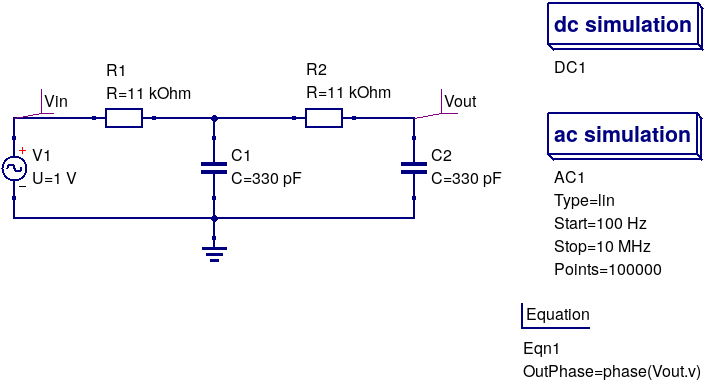
\includegraphics[width = 400pt]{images/qucs-scheme.png}
\caption{Scheme from Qucs}
\label{fig:qucs_scheme}
\end{figure}

\begin{figure}[h!]
\centering
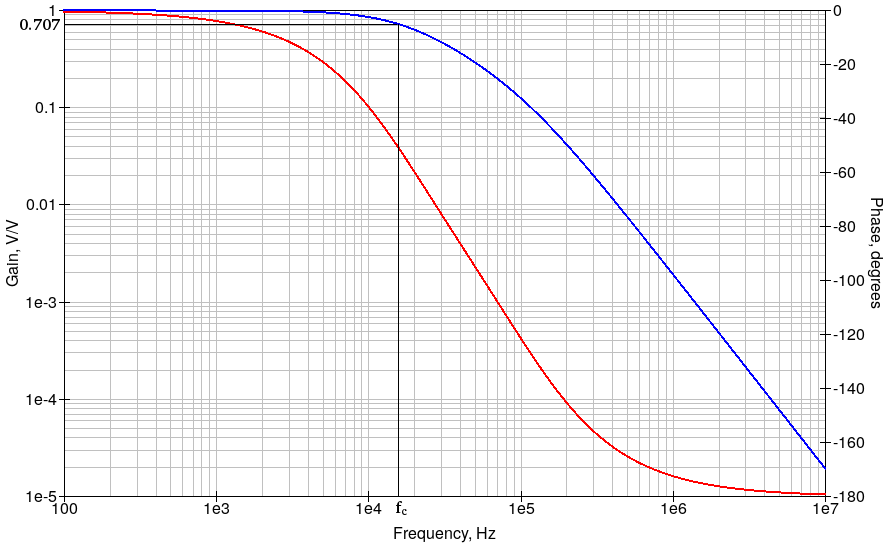
\includegraphics[width = 420pt]{images/qucs-plot.png}
\caption{Plot from Qucs}
\label{fig:qucs_plot}
\end{figure}

\end{document}
